\documentclass{article}

\usepackage{amsmath}
\usepackage{geometry}
\usepackage{amscd}
\usepackage[tableposition=top]{caption}
\usepackage{ifthen}
\usepackage[utf8]{inputenc}

\usepackage{Sweave}


\begin{document}

\title{The \textbf{tvtools} package for R}
\author{David Shilane}
\maketitle

\noindent The \textbf{tvtools} software package is designed to aid in the analysis of long--form time--varying (LFTV) data structures.  Long--form data allows for each subject in the study to have multiple rows of information.  Each row of data corresponds to the subject's status in a specific time interval.  Applications such as medical studies may include dozens or hundreds of records for each of tens of thousands of patients.  As such, a time--varying data structure is vastly larger than a typical baseline study.  Furthermore, the introduction of a time axis adds complexity to the typical descriptive statistics, tables, and figures used to explore the data set.  The \textbf{tvtools} package provides a variety of methods to aid in the description and visualization of long--form time--varying data.

\section{Long--form time--varying data}

Let's consider the following (artificial) example of an LFTV data set:

% latex table generated in R 2.12.2 by xtable 1.5-6 package
% Sun Dec 25 00:24:32 2011
\begin{table}[ht]
\begin{center}
\begin{tabular}{rrrrrrr}
  \hline
 & ID & time1 & time2 & age & drug & death \\ 
  \hline
Row 1 & 1 & 0 & 5 & 65 & 1 & 0 \\ 
  Row 2 & 1 & 5 & 6 & 65 & 1 & 1 \\ 
  Row 3 & 2 & 0 & 3 & 60 & 1 & 0 \\ 
  Row 4 & 2 & 3 & 10 & 60 & 0 & 0 \\ 
  Row 5 & 2 & 10 & 12 & 60 & 1 & 0 \\ 
  Row 6 & 3 & 0 & 8 & 70 & 0 & 0 \\ 
  Row 7 & 3 & 8 & 9 & 70 & 1 & 1 \\ 
  Row 8 & 4 & 0 & 2 & 85 & 0 & 1 \\ 
  Row 9 & 5 & 0 & 6 & 55 & 1 & 0 \\ 
  Row 10 & 5 & 6 & 15 & 55 & 0 & 0 \\ 
   \hline
\end{tabular}
\caption{Example of a LFTV data set.}
\label{ex1}
\end{center}
\end{table}
\noindent Each row includes the following information:

\begin{itemize}
\item \textbf{An ID field}:  This ensures that a subject with multiple rows will have all of its information linked together by the identification variable.

\item \textbf{Time intervals}:  Each row represents the subject's status in a specific interval of time.  The left and right endpoints of this interval are given by the variables \textbf{time1} and \textbf{time2}, respectively.  Other names may be substituted.  In general, the time intervals for a given subject must be mutually exclusive.  In most cases, they will also be collectively exhaustive.  The first time interval for each subject typically begins at 0, and the last interval typically ends at the maximum follow--up time for the subject.  We will assume that the subject's status changes instantaneously at the left end--point of each interval from the previous to the current status.  Moreover, this status will remain fixed for the duration of the time interval.

\item \textbf{Baseline covariates}:  Some variables are measured only a single time (e.g. at baseline) or are otherwise unchanging.  The LFTV data structure repeats these variables with the same value in each row.

\item \textbf{Time--varying data}:  These variables may change within each time interval.  Depending upon the context, some variables have limits on how they may change with time.  For instance, in survival analyses, a measure of mortality may change from 0 to 1 but not back.  Other outcomes may repeatedly alternate between states.  In medical studies, the time of certain events (e.g. myocardial infarction) may be recorded.  These variables will take the value 1 at the time of the event and then return to 0 in the next time interval.

\end{itemize}

\noindent The example in Table \ref{ex1} depicts a study examining the effect of age and a drug on survival.  In this case, the time units are in months.  The first patient entered the study at age 65, was treated with the drug, and survived for 5 months.  The second patient entered the study at age 60, received 3 months of drug treatment, spent months 3--10 off of the drug, reinitiated the treatment from months 10--12, and survived at least until the end of the 12 month follow--up.\\

\noindent The stories of each patient are easy enough to understand if you read through each row.  However, some very simple questions are more difficult to answer with the basic tools of descriptive analysis.  For instance, we might ask:

\begin{itemize}
\item What was the average drug exposure for each patient?  This would be the number of months on treatment divided by the overall number of months each patient was observed.  However, since patients are followed over multiple rows, the follow--up time must be identified, and the treatment variable must be weighted in each row by the length of the time interval.

\item What was the death rate for patients on and off of the drug?  The number of deaths in each category may be counted up within the subset of rows on and off the drug treatment.  Then these counts must be weighed against the overall time of exposure.  That is, instead of simply saying that a certain percentage survived past 6 months, we must provide an answer in terms of survival per person per month.

\item How soon do patients tend to die after initiating the drug treatment?  We must first identify the time that each patient started the drug (if ever).  Then we may compare this date to the time of death. 
\end{itemize}

\noindent Each of these questions has a temporal nature in addition to the usual statistical questions of rates or averages.  The usual tools of descriptive statistics require some augmentation to arrive at the proper answer.  The \textbf{tvtools} package seeks to provide effective methods for solving these problems.

\noindent The goals of the \textbf{tvtools} package are:

\begin{enumerate}
\item \textbf{Compute crude rates} of exposure and event occurrences.  This may include:

\begin{itemize}
\item \textbf{Cross-sectional rates:}  This can be the percentage of the population with a certain condition at a specific time.  Note that time intervals beyond some patients' length of follow--up will be accounted for.

\item \textbf{Event rates relative to exposure:}  This will compute factors such as the death rate per person year of follow-up.

\item \textbf{Event rates relative to exposure and split by treatment category:}  This will compute factors such as the death rate per person year on and off of drug treatment.
\end{itemize}

\textbf{Implemented in cruderates.R}

\item Compute time to events.  \textbf{Implemented in firstevent.R}

\item Compute overall time of follow--up for each patient.  \textbf{Implemented in followuptime.R}

\item Compute rate of exposure over a specific time frame.  (E.g. the percentage of days exposed to drug treatment in the first year.)  \textbf{Implemented in exposure.R}

\item Create treatment exposure graphics:
\begin{itemize}
\item Depict drug exposure timelines for multiple simultaneous treatments.

\item Display timelines of events

\end{itemize}

\textbf{Implemented in timeplot.R}

\item Create a cross-sectional data set at a specific time.  For baseline data sets, include the time to specified events.  \textbf{Implemented in create.baseline.R.}

\item Account for the degree of missingness in a variable at specific time points.  \textbf{Implemented in missingness.R.}


\end{enumerate}

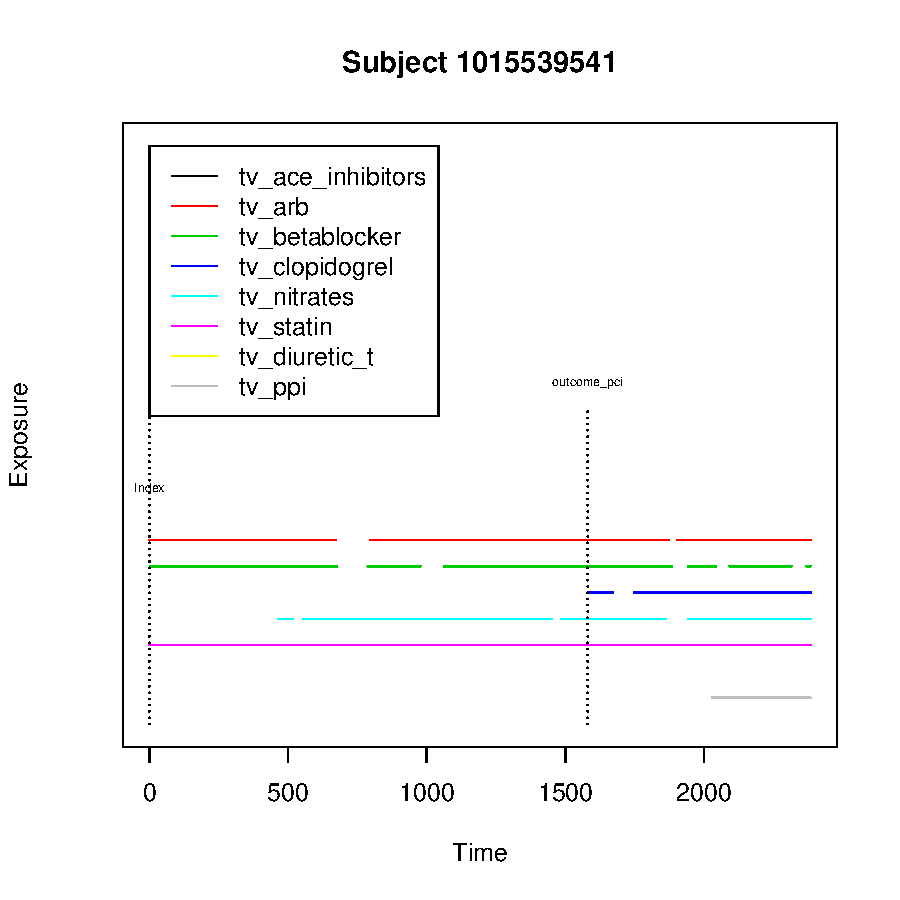
\includegraphics{plans-tab2}

\end{document}
